\section{Thermal review}

	\subsection{Heat zones in machining}
	\label{subsec:heatzones}

	In machining there are 3 main regions of interest from where comes the heat produced during the cutting process \cite{shaw2005metal}. The first area represented on figure \ref{fig:heatZones} is called primary shear zone and it is located along the shear plane, which is the boundary between undeformed workpiece and chip. The second area is the contact plane between tool and chip, also known as secondary shear zone or friction zone. As for the third one, it is related to the wear caused due to the friction between tool and finished workpiece surface. It is called wear zone or tertiary zone.

	\begin{figure}[h]
		\centering
		\captionsetup{justification=centering}
		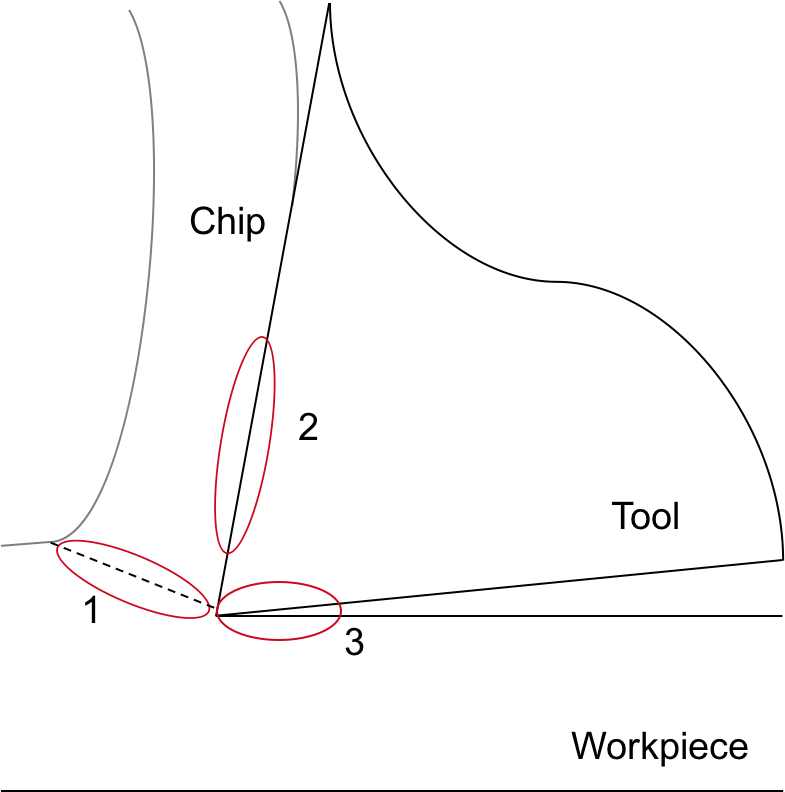
\includegraphics[scale=0.5]{Imagens/heatZones.png}
		\caption{Regions of interest during tool-chip interaction}
		\label{fig:heatZones}
	\end{figure}

	All the heat generated in these three zones is removed from the system by means of tool, chip and workpiece. Since the cutting velocities used in this study are high, the cutting process is classified as high speed machining. The process is more adiabatic as the cutting velocity raises because of the short process time prevents the heat of being dissipated from the heat source directly to the environment. 

	It is important to highlight that the heat generation on primary and secondary shear zones is highly influenced by the cutting conditions, while for the tertiary zone is mainly dependent on tool flank wear \cite{abukhshim2006heat}. In this study, each cutting experiment was performed with sharp tools, so that the wear zone had a minor influence on total heat generation \cite{shaw2005metal}.

	\subsection{Fundamentals of heat transfer}

	Heat transfer occurs in three basic ways: Conduction, convection and radiation. Each situation can present one or more of these modes happening at the same time \cite{poole1989fundamentals}. Regarding conduction, this is a mechanism in which heat is transferred from a region with high temperatures to another region with lower temperatures in a material. The general equation for heat conduction in three dimensions is given by:

	\begin{equation} 
	\label{}
	k(\frac{\partial ^{2}T}{\partial x^{2}} + \frac{\partial ^{2}T}{\partial y^{2}} + \frac{\partial ^{2}T}{\partial z^{2}}) + q = \rho c_{p}\frac{\partial T}{\partial t}
	\end{equation}

	Where $q$ is the heat generated per volume, $k$ is the heat conductivity, $T$ is temperature, $t$ is time, $\rho$ is the density of the material, $c_{p}$ is the specific heat capacity and $x$, $y$ and $z$ are the directions of heat propagation.

	Convection is the way of heat propagation between bodies and fluids and within fluids. It happens because of density difference caused by the temperature difference. The equation that rules this mode is:

	\begin{equation} 
	\label{}
	q = h_{c}A(T_{f} - T{s})
	\end{equation}

	Where $h_{c}$ is the convective heat transfer coefficient, $A$ is the area of the body in contact with the fluid and $T_{f}$ and $T_{s}$ are the temperatures of the fluid and surface, respectively.

	For the third mode, the presence of a transport medium is not necessary. Radiation makes it possible for heat transfer in vacuum and any body above absolute zero emits electromagnetic energy causing heat propagation. Given two bodies with absolute temperatures $T_{1}$ and $T_{2}$, the heat propagation is:

	\begin{equation} 
	\label{}
	q = \epsilon \sigma_{B}A(T_{1}^{4} - T_{2}^{4})
	\end{equation}

	$\sigma_{B}$ is the Stefan-Boltzmann constant, $\epsilon$ is the emissivity and $A$ is the enclosed area of the body.

	Besides radiation, which comes to be the prevailing mode in infrared thermography, which will be discussed on the following subsection \ref{subsec:infraOp}, the focus of this paper is in the conduction transfer present in the cutting zone.

	\subsection{Infrared thermography operation}
	\label{subsec:infraOp}

	Infrared termography is a non-contact way of measuring infrared electromagnetic energy. The human eye cannot detect the range of infrared radiation. However, there are infrared cameras which are able to detect this energy and process the radiation into visual information (figure \ref{fig:thermog}).

	\begin{figure}[H]
		\centering
		\captionsetup{justification=centering}
		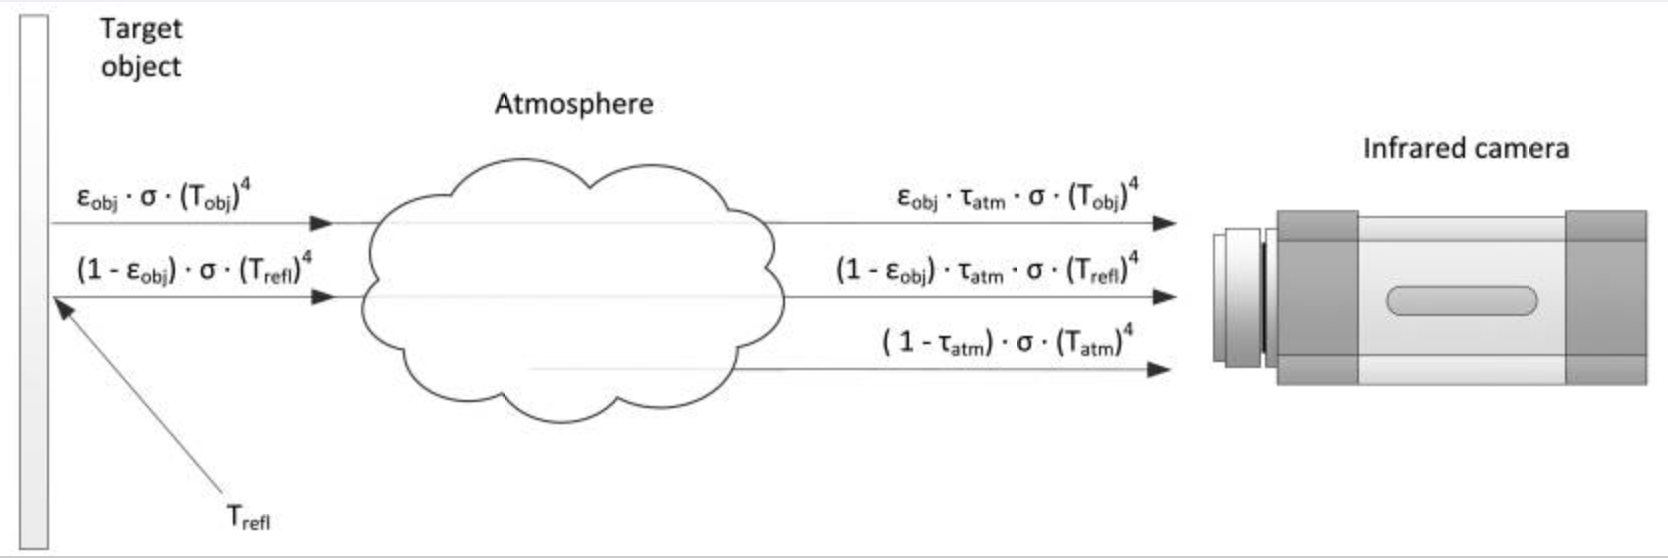
\includegraphics[scale=0.5]{Imagens/thermography.png}
		\caption{Radiation received by infrared camera \cite{usamentiaga2014}}
		\label{fig:thermog}
	\end{figure}

	It makes it possible for all thermal energy produced during a cutting process to be received by the infrared camera and to be later synthesize into a temperature matrix. Since every body is able to emit infrared radiation when its temperature is above absolute zero, it is possible to observe contours of different bodies due to their temperature distribution. For this reason, thermography is a very important technology in military use, because it allows objects to be seen even without proper illumination or in total lack of light situations.

	Thermography is able to work in two different ways: passive and active. The passive variety occurs when the subject has its temperature different from the environment (often higher). On the other hand, active thermography needs an external heat source to induce a reasonable contrast between the object and the background \cite{maldague2000}.

	As it can be observed on Figure \ref{fig:thermog}, there are external sources of infrared radiation that can interfere in the target's temperature measurement. To correct this situation, the IR camera has an internal process called compensation \cite{usamentiaga2014}.

	The total energy received ($W_{tot}$) is composed by the sum of three parts: the emission from the main object ($E_{obj}$), the emission of the vicinity reflected by the object ($E_{refl}$) and the emission of the atmosphere ($E_{atm}$) as shown on figure \ref{fig:thermog}. Then it is possible to extract the real temperature of the target object \cite{usamentiaga2014}.


\section{Mechanical review}
	\subsection{Mechanics of orthogonal cutting}

	In this section it will be shown innumerous relations among forces, stresses and dimensions, for example. For this purpose it is important to discuss geometrical correlations in the composite cutting force circle (figure \ref{fig:circlec}).

	\begin{figure}[h]
		\centering
		\captionsetup{justification=centering}
		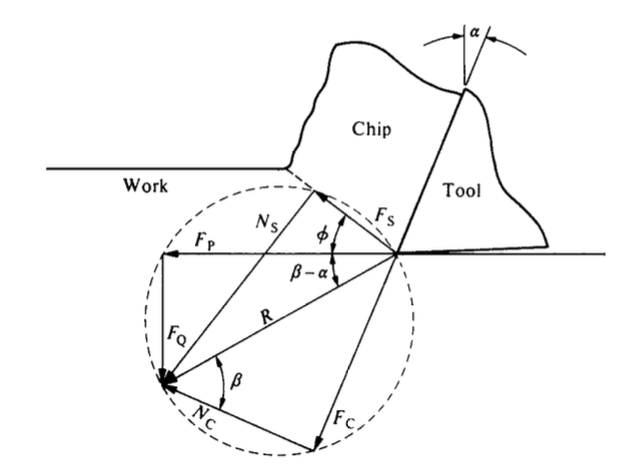
\includegraphics[scale=0.5]{Cap1/circlec.png}
		\caption{Cutting forces \cite{shaw2005metal}}
		\label{fig:circlec}
	\end{figure}

	From the figure \ref{fig:circlec} it can be stated about forces on the primary shear zone reference $F_{S}$ and $N_{S}$:

	\begin{equation} 
	\label{}
	F_{S} = F_{P}\cos\phi - F_{Q}\sin\phi
	\end{equation}

	\begin{equation} 
	\label{}
	N_{S} = F_{Q}\cos\phi + F_{P}\sin\phi
	\end{equation}

	Also, for the forces on the chip flow direction reference:

	\begin{equation} 
	\label{}
	F_{C} = F_{P}\sin\alpha + F_{Q}\cos\alpha
	\end{equation}

	\begin{equation} 
	\label{}
	N_{C} = F_{P}\cos\alpha - F_{Q}\sin\alpha
	\end{equation}

	These equations provide all auxiliary forces related to the known passive force $F_{Q}$ and the force on the cutting direction $F_{P}$. Now the variables of interest can be easily calculated, such as the friction coefficient:

	\begin{equation} 
	\label{eq_friction}
	\mu = \frac{F_{C}}{N_{C}} = \frac{F_{Q} + F_{P}\tan\alpha}{F_{P} - F_{Q}\tan\alpha}
	\end{equation}

	The equations concerning stresses are:

	\begin{equation} 
	\label{}
	A_{S} = \frac{wa_{p}}{\sin\phi}
	\end{equation}

	\begin{equation} 
	\label{}
	\tau = \frac{F_{S}}{A_{S}} = \frac{(F_{P}\cos\phi - F_{Q}\sin\phi)\sin\phi}{wa_{p}}
	\end{equation}

	\begin{equation} 
	\label{}
	\sigma = \frac{N_{S}}{A_{S}} = \frac{(F_{P}\sin\phi + F_{Q}\cos\phi)\sin\phi}{wa_{p}}
	\end{equation}

	Where $A_{S}$ is the area of the shear plane, $\tau$ is the shear stress and $\sigma$ is the normal stress.

	Another important parameter is the cutting ratio $r$, which can provide an important relation between the main cutting velocity and the chip outlet velocity. It has been found experimentally that there is no change in density of metal during the cutting process and also that $w/a_{p} \geq 5$ makes the width of the chip the same than that of the workpiece. Thus, the equations are:

	\begin{equation} 
	\label{}
	a_{p}wl = a_{pc}w_{c}l_{c}
	\end{equation}

	Where $a_{p}$, $w$ and $l$ are the depth of cut, width of cut and length of cut, respectively. Then, the cutting ratio is defined by:

	\begin{equation} 
	\label{}
	r = \frac{a_{p}}{a_{pc}} = \frac{l_{c}}{l}
	\end{equation}

	With the cutting ratio, it is now possible to correlate cutting velocity $v$ and chip outlet velocity $v_{c}$ by means of the following equation:

	\begin{equation} 
	\label{}
	v_{c} = rv
	\end{equation}

\section{State of the Art}

\subsection{Infrared Termography}
	\label{sec:infrared}
		For the use of infrared thermography it can be found studies for inspection application. The infrared camera makes possible to work with thermal information in entire areas covered by the field of view, different from thermocouples that are able to measure punctual temperatures for example.

	\citeonline{lee2011study} shows a study on integrity of resistance spot welding by means of infrared thermography. It was set two external heat sources in order to raise the temperature of the spot. The results have shown a promising method of inspection when comes to diameter measurement of the nugget. While measurements made with naked eye provide a difference of about 20\%, the thermography provides only 8\%.

	\begin{figure}[H]
		\centering
		\captionsetup{justification=centering}
		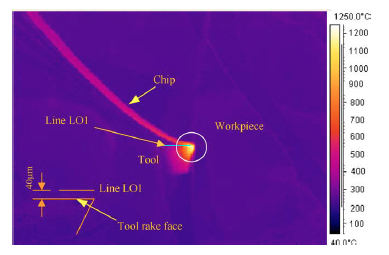
\includegraphics[scale=0.75]{Cap2/InfraRed/exinfrared.png}
		\caption{Infrared photography of a cutting process \cite{abukhshim2006heat}}
		\label{fig:exinfrared}
	\end{figure}

	For the case under study, high speed thermography has its positive and negative points. On the positive side, it may be mentioned:

	\begin{itemize}
		\item Fast inspection rate (reasonable number of images of high speed cutting)
		\item Contactless (no interference during the cutting process)
		\item Easy interpretation of the results (indexed image with temperatures in each pixel)
	\end{itemize}

	But it is also important to mention the difficulties that in this method still prevail:
	
	\begin{itemize}
		\item Only a limited thickness can be measured (under the main surface)
		\item Determine a suitable emissivity is a chalenge (it changes with temperature variation)
	\end{itemize}
 %done

\subsection{Image Processing}
	Systems of vision have been very often approached with the current fast technology development and intelligent systems. They are used for the most diverse segments, as military and medical areas. Image processing has quickly gaining highlight. For instance, this is essential when comes to finding a pattern or extract an specific feature in a image. 

Colorful or gray scaled images can be treated as matrices with dimensions given by their pixel resolution. Each pixel corresponds to a cell inside this matrix and each cell contains a relevant information, it could be a level in grayscale, a coordinate or a temperature as in the case of this paper. Since they are matrices, they can be easily manipulated by means of mathematical operations and, consequently, processed to highlight one specific property or more.

Many studies have been and are being done about the use of image processing on machining. It was used to monitor flank wear of cutting tools \cite{jeon1988optical}, \cite{kurada1997machine} and also for detection of chatter during cutting processes \cite{khalifa2006image}. These are few examples of what image processing can do for machining industry, increasing tool life and surface finishing. There are uncountable ways which this tool can be applied to improve processes and quality of final products. The fast development of computer hardware makes the processing time of images continuously shorter, allowing systems of vision to be incorporated in online monitoring and then providing a real time feedback.
